\documentclass[12pt,a4paper]{article}
\usepackage[utf8]{inputenc}
\usepackage[francais]{babel}
\usepackage[T1]{fontenc}
\usepackage{amsmath}
\usepackage{amsfonts}
\usepackage{amssymb}
\usepackage{listings}
\usepackage{xcolor}
\usepackage{graphicx}

\usepackage{authblk}


\graphicspath{{./ROC1.jpg}}
\graphicspath{{./ROC1.jpg}}
\graphicspath{{./ROC1.jpg}}

\definecolor{codegreen}{rgb}{0,0.6,0}
\definecolor{codegray}{rgb}{0.5,0.5,0.5}
\definecolor{codepurple}{rgb}{0.58,0,0.82}
\definecolor{backcolour}{rgb}{0.95,0.95,0.92}

\lstdefinestyle{mystyle}{
    backgroundcolor=\color{backcolour},   
    commentstyle=\color{codegreen},
    keywordstyle=\color{magenta},
    numberstyle=\tiny\color{codegray},
    stringstyle=\color{codepurple},
    basicstyle=\ttfamily\footnotesize,
    breakatwhitespace=false,         
    breaklines=true,                 
    captionpos=b,                    
    keepspaces=true,                 
    numbers=left,                    
    numbersep=5pt,                  
    showspaces=false,                
    showstringspaces=false,
    showtabs=false,                  
    tabsize=2
}

\lstset{style=mystyle}
\title{TP 1 Mesures de performance}


\author{Rahiche Messaoud | Groupe 3 \and Krizou Amani | Groupe 3 \and Adda Redouane | Groupe 3 \and Mendil Yousra | Groupe 3 }

\renewcommand\Authands{ and }
\date{ }
\begin{document}
\maketitle
\newpage
\tableofcontents

\newpage
\section{KNN}
\subsection{L'implémentation de l'Algorithme}
\begin{enumerate}
\item \underline{Pseudo code:}
	\begin{itemize}
	\item Charger les données
	\item Initialiser la valeur de k.
	\item Calculez la distance entre les données de test et chaque ligne de données d'entraînement.
	\item Trier les distances calculées par ordre croissant en fonction des valeurs de distance.
	\item Obtenir les k premières lignes du tableau trié
	\item Obtenir la classe la plus fréquente de ces lignes
	\item Renvoie la classe prédite
	\end{itemize}
\item \underline{Python code:}
\begin{lstlisting}[language=Python]
def euc_dist(x1, x2):
    return np.sqrt(np.sum(x1-x2)**2)

def KPP(x,Xt,Yt):
    predicted_labels = [predict(x)]
    return np.array(predicted_labels)

def predict(x):
    k=10
    distances = np.array([euc_dist(x, xt) for xt in Xt])
    
    #get the k nearest neighbors and labels:
    kdist = distances.argsort()[0:k]
    knear = [Yt[i] for i in kdist]
    
    #Illustrating the k-nearest neighbor:
    plt.figure(figsize=(20,10))
    for i in range(10):
        d= Xt[kdist[i],:].reshape((20, 20))
        d=np.transpose(d)
        plt.subplot(1,10,i+1)
        plt.title('label '+ str(Yt[kdist[i]]))
        plt.imshow(d,cmap='gray')
        
    #majority vote:
    majority = Counter(knear).most_common(1)
    return majority
\end{lstlisting}

\end{enumerate}

\subsection{Matrice de confusion:}
On a fait l'affichage de la matrice de confusion de chaque classe dans le fichier jupyter, alors ici on a cree un tableau qui les regroupe:
\begin{center}
\scalebox{0.9}{
\begin{tabular}{| c | c | c | c | c | c | c | c | c | c | c |}
\hline
Classe & 0 & 1 & 2 & 3 & 4 & 5 & 6 & 7 & 8 & 9 \\
\hline
VP & 196 & 266 & 122 & 126 & 140 & 127 & 145 & 142 & 135 & 150\\
\hline
VN & 2765 & 2878 & 2841 & 2854 & 2799 & 2859 & 2792 & 2847 & 2777 & 2801\\
\hline
FP & 241 & 112 & 169 & 151 & 206 & 140 & 193 & 157 & 217 & 198 \\
\hline
FN & 131 & 77 & 201 & 202 & 188 & 207 & 203 & 187 & 204 & 184\\
\hline
\end{tabular}}
\end{center}

\subsection{Le rappel, La precision et Le taux de faux positif:}
Le tableau suivant englobe les mesures de performance de chaque classe:
\begin{center}
\scalebox{0.9}{
\begin{tabular}{| c | c | c | c | c | c | c | c | c | c | c |}
\hline
Classe & 0 & 1 & 2 & 3 & 4 & 5 & 6 & 7 & 8 & 9 \\
\hline
Rappel & 0.599 & 0.775 & 0.377 & 0.384 & 0.426 & 0.380 & 0.416 & 0.431 & 0.398 & 0.449\\
\hline
Précision & 0.448 & 0.703 & 0.419 & 0.454 & 0.404 & 0.475 & 0.428 & 0.474 & 0.383 & 0.431\\
\hline
Taux de FP & 0.448 & 0.592 & 0.456 & 0.427 & 0.522 & 0.403 & 0.487 & 0.456 & 0.515 & 0.518 \\
\hline
\end{tabular}}
\end{center}

\newpage

\section{MVS}
\subsection{Courbe ROC:}
\begin{center}
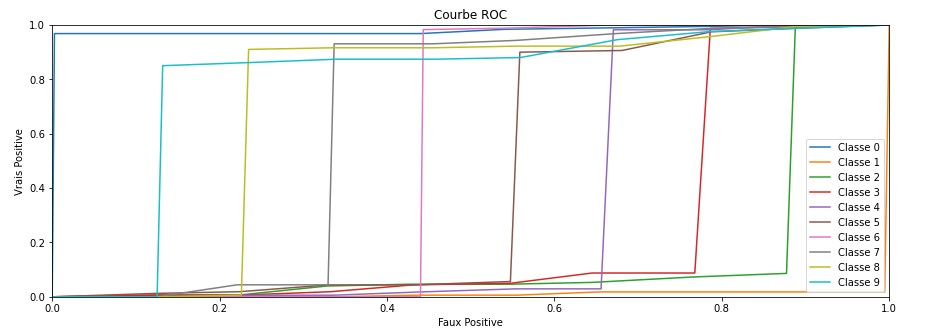
\includegraphics[scale=0.6]{ROC1.jpg}
\end{center}


\subsection{Matrice de confusion:}
On a fait l'affichage de la matrice de confusion de chaque classe dans le fichier jupyter, alors ici on a cree un tableau qui les regroupe:
\begin{center}
\scalebox{0.9}{
\begin{tabular}{| c | c | c | c | c | c | c | c | c | c | c |}
\hline
Classe & 0 & 1 & 2 & 3 & 4 & 5 & 6 & 7 & 8 & 9 \\
\hline
VP & 184 & 163 & 137 & 144 & 163 & 135 & 173 & 141 & 151 & 142\\
\hline
VN & 1473 & 1493 & 1500 & 1479 & 1474 & 1490 & 1486 & 1497 & 1487 & 1490\\
\hline
FP & 6 & 3 & 14 & 16 & 8 & 25 & 3 & 18 & 16 & 25 \\
\hline
FN & 4 & 8 & 16 & 28 & 22 & 17 & 5 & 11 & 13 & 10\\
\hline
\end{tabular}}
\end{center}

\subsection{Le rappel, La precision et Le taux de faux positif:}
Le tableau suivant englobe les mesures de performance de chaque classe:
\begin{center}
\scalebox{0.9}{
\begin{tabular}{| c | c | c | c | c | c | c | c | c | c | c |}
\hline
Classe & 0 & 1 & 2 & 3 & 4 & 5 & 6 & 7 & 8 & 9 \\
\hline
Rappel & 0.968  & 0.981 & 0.907 & 0.9 & 0.953 & 0.843 & 0.982 &  0.886 & 0.904 & 0.850 \\
\hline
Précision & 0.978 & 0.953 & 0.895 & 0.837 & 0.881 & 0.888 & 0.971 & 0.927 & 0.920 & 0.934  \\
\hline
Taux de FP & 0.4 & 0.727 & 0.533 & 0.636 &  0.733 & 0.404 & 0.625 & 0.379 &0.448 & 0.285 \\
\hline
\end{tabular}}
\end{center}

\newpage

\section{Arbres de décision}
\subsection{Courbe ROC:}
\begin{center}
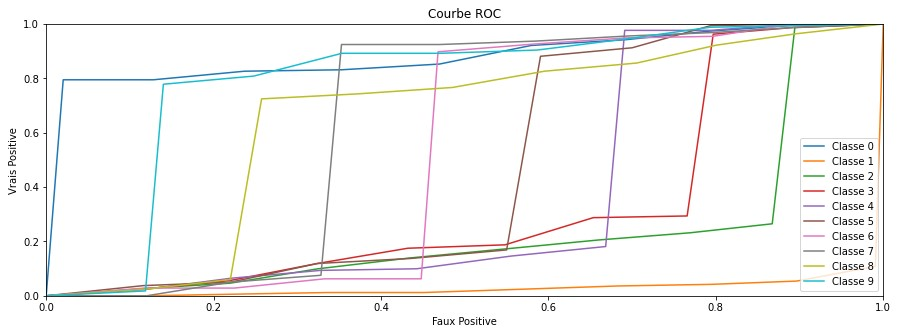
\includegraphics[scale=0.6]{ROC2.jpg}
\end{center}

\subsection{Matrice de confusion:}
On a fait l'affichage de la matrice de confusion de chaque classe dans le fichier jupyter, alors ici on a cree un tableau qui les regroupe:
\begin{center}
\scalebox{0.9}{
\begin{tabular}{| c | c | c | c | c | c | c | c | c | c | c |}
\hline
Classe & 0 & 1 & 2 & 3 & 4 & 5 & 6 & 7 & 8 & 9 \\
\hline
VP & 151 & 148 & 109 & 107 & 136 &  114 & 147 & 135 & 111 & 127 \\
\hline
VN & 1447 & 1487 & 1475 & 1460 & 1462& 1446 & 1461 & 1471 & 1444  & 1468  \\
\hline
FP & 39 & 18 & 42 & 53 & 35 & 46 & 29 & 24 & 56 & 40 \\
\hline
FN & 30 & 14 & 41 & 47 & 34 & 61 & 30 & 37 & 56 & 32 \\
\hline
\end{tabular}}
\end{center}

\subsection{Le rappel, La precision et Le taux de faux positif:}
Le tableau suivant englobe les mesures de performance de chaque classe:
\begin{center}
\scalebox{0.9}{
\begin{tabular}{| c | c | c | c | c | c | c | c | c | c | c |}
\hline
Classe & 0 & 1 & 2 & 3 & 4 & 5 & 6 & 7 & 8 & 9 \\
\hline
Rappel & 0.794 & 0.891 & 0.721 &  0.668 & 0.795 &  0.7125 & 0.835 &  0.849 & 0.664 & 0.760 \\
\hline
Précision &  0.834 & 0.913 & 0.726 & 0.694 & 0.8 & 0.651 & 0.830 & 0.784 & 0.664 & 0.798 \\
\hline
Taux de FP & 0.434 & 0.4375 & 0.493 & 0.47 & 0.492 & 0.570 & 0.508 & 0.606 &  0.5 & 0.444 \\
\hline
\end{tabular}}
\end{center}


\newpage

\section{Réseaux de neurones Perceptron}
\subsection{Courbe ROC:}
\begin{center}
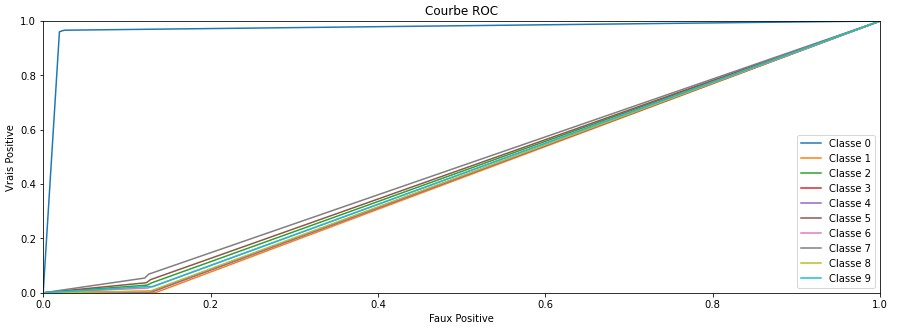
\includegraphics[scale=0.6]{ROC3.jpg}
\end{center}

\subsection{Matrice de confusion:}
On a fait l'affichage de la matrice de confusion de chaque classe dans le fichier jupyter, alors ici on a cree un tableau qui les regroupe:
\begin{center}
\scalebox{0.9}{
\begin{tabular}{| c | c | c | c | c | c | c | c | c | c | c |}
\hline
Classe & 0 & 1 & 2 & 3 & 4 & 5 & 6 & 7 & 8 & 9 \\
\hline
VP & 146 & 0 & 0 & 0 & 156 & 0 & 0 & 3 & 0 & 0 \\
\hline
VN & 1491 & 1503 & 1504 & 1497 & 179 & 1485 & 1505 & 1491 & 1481 & 1505 \\
\hline
FP & 6 & 164 & 163 & 170 & 1 & 182 & 162 & 166 & 186 & 162 \\
\hline
FN & 24 & 0 & 0 & 0 & 1331 & 0 &  0 & 7 & 0 &  0\\
\hline
\end{tabular}}
\end{center}

\subsection{Le rappel, La precision et Le taux de faux positif:}
Le tableau suivant englobe les mesures de performance de chaque classe:
\begin{center}
\scalebox{0.9}{
\begin{tabular}{| c | c | c | c | c | c | c | c | c | c | c |}
\hline
Classe & 0 & 1 & 2 & 3 & 4 & 5 & 6 & 7 & 8 & 9 \\
\hline
Rappel & 0.960  & 0.0 & 0.0 & 0.0 & 0.993 & 0.0 & 0.0 & 0.017 & 0.0 & 0.0 \\
\hline
Précision & 0.858 & / & / & / & 0.104 & / & / & 0.3 & / & / \\
\hline
Taux de FP & 0.8 & 0.0 & 0.0 & 0.0 & 0.999 & 0.0 & 0.0 & 0.040 & 0.0 & 0.0 \\
\hline
\end{tabular}}
\end{center}




\end{document}